\chapter{From positive states to a unitary theory}
\label{ch:unitarity}

The lattice construction begins in a positive Hilbert space. Why,
then, is a separate chapter on unitarity necessary? The answer is
that the vacuum representation is only one part of a rational CFT.
Other modules describe charged sectors, and intertwining operators
describe their fusion. Positivity must be compatible with all of
these structures. An abstract equivalence of fusion rules, or even
of braided categories without specified positive structures, does
not automatically establish this compatibility for the actual VOA
operators.

This chapter explains the analytic route used in the construction.
The model-specific inputs are the regularity and branching results
of Part II and the twelve-module count. Standard comparison theorems
for lattice VOAs, conformal nets, and annulus insertions supply the
analytic framework. We prove the elementary domain lemmas in full
and describe how the remaining comparison fits together. The account
retains the research manuscript's finite-input qualifications.

\section{Three levels of unitarity}
\index{unitarity!vacuum}\index{unitarity!strong}\index{unitarity!complete}

\emph{Vacuum unitarity} means that $U$ itself has a positive
invariant Hermitian form and the corresponding antilinear PCT
involution. This follows here from PCT stability inside the positive
lattice theory.

\emph{Strong unitarity} means that every simple ordinary $U$-module
admits a positive invariant Hermitian form. It is a statement about
all sectors, including ones not explicitly visible as subspaces of
the original lattice vacuum.

\emph{Complete unitarity} additionally requires positivity of the
canonical Hermitian forms on fusion, or intertwining-operator,
spaces. It gives the VOA representation category its unitary
modular tensor structure. Choosing positive norms separately on
the simple modules does not prove this last condition: the
associativity and braiding operators must also be compatible with
the fusion pairings.

A finite-dimensional analogy is helpful. Giving each vector space
in a diagram an inner product does not make every linear map in
the diagram unitary. Nor can arbitrary independent changes of
metric be assumed to respect a collection of tensor products and
composition laws. Fusion positivity is the corresponding
compatibility problem for chiral fields.

\section{Why smeared fields lead to operator algebras}
\index{conformal net}\index{smeared field}\index{energy bound}\index{strong locality}

An individual field $Y(v,z)$ is usually unbounded and may not define
an operator on every vector of the Hilbert completion. To obtain a
well-controlled operator, smear it against a smooth function on the
circle:
\[
 Y(v,f)=\sum_n\widehat f_n\,v_{(n)},
\]
with the indexing adjusted to the chosen circle convention.
Polynomial energy bounds have the schematic form
\begin{equation}
 \norm{v_{(n)}\xi}
 \le C(1+|n|)^s\norm{(1+L_0)^r\xi}
 \label{eq:unitarity-energy-bound}
\end{equation}
on finite-energy vectors. Smooth Fourier coefficients decay faster
than any power, so these estimates permit smearing on a dense
domain and then taking the closure.

A \emph{conformal net} assigns to every interval $I$ of the circle
a von Neumann algebra $\mathcal N(I)$ of bounded observables.
Inclusions of intervals give inclusions of algebras, disjoint
intervals give commuting algebras, and conformal transformations
transport the assignment. The vacuum is cyclic, and rotations have
positive energy. A von Neumann algebra is an algebra of bounded
operators closed under adjoints and weak operator limits.

For a strongly local unitary VOA, the closed smeared fields generate
such a net. An unbounded operator can be affiliated with a von
Neumann algebra through the bounded operators in its polar
decomposition and its spectral projections. Strong locality is
the analytic statement that the algebras associated with disjoint
supports commute; formal OPE locality alone must not silently be
substituted for it.

Lattice VOAs satisfy the required locality and energy properties,
and the relevant unitary subalgebra inheritance theorems apply to
$U\subset B\subset H=V_{E_8}$. Since all three share the ambient
conformal vector, they also share the rotation generator on their
vacuum spaces and central charge eight.

\section{Sectors, statistical dimension, and complete rationality}
\index{complete rationality}\index{statistical dimension}

A sector is a representation of the local observable algebras that
is compatible with their inclusions. In the chiral net setting,
localized transportable representations admit fusion, statistical
dimensions, and braiding. These are the operator-algebraic
counterparts of VOA modules and their tensor products.
Localized means equivalent to the vacuum outside a chosen interval;
transportable means that the charge can be relocated to any other
interval by an equivalent representation.

For a finite-index sector realized by a localized endomorphism
$\sigma$, the statistical dimension can be defined through
the local inclusion
\[
 d(\sigma)^2=
 [\,\mathcal N(I):\sigma(\mathcal N(I))\,].
\]
Here $I$ contains the localization region and the index has
the standard minimal-index normalization. Thus the statistical
dimension is a square root of an operator-algebra index, rather
than the number of vectors in the sector's Hilbert space.

A completely rational net satisfies suitable split and strong
additivity conditions and has finite two-interval index. The split
property expresses a controlled independence of observables in
separated intervals. Strong additivity says that removing one point
from an interval does not lose its generated observable algebra.
Under these conditions, the sectors form a unitary modular tensor
category, and the two-interval index is
\[
 \mu(\mathcal N)=\sum_i d_i^2.
\]
A holomorphic net has only its vacuum sector and $\mu=1$.

There is a second way to form the local algebras, using point
insertions regularized by incoming and outgoing annuli.
Its hypothesis is called \emph{bounded localized vertex operators}.
For each allowed insertion $z$ between annuli $A,B$, one requires
some $0<s<1$ for which
\[
 v\otimes\xi\longmapsto BY(s^{L_0}v,z)A\xi
\]
extends to a bounded operator on the Hilbert tensor product.
This controls the inserted state as well as the vector on which
the field acts. The local algebras generated by these insertions
and by the no-insertion products $BA$ must commute for disjoint
intervals. The lattice theory has this property, and the unitary
subalgebra inherits it. The annulus section below explains the
geometry and its module counterpart.

The construction first obtains complete rationality through a
bounded-insertion version of the subnet. Regularity of $U$ and
the lattice ambient theory imply finite index for this inclusion;
finite index in a holomorphic completely rational net then implies
complete rationality of the subnet. A vacuum-net comparison carries
that property to the net generated by smeared fields.

At this stage only an isomorphism-invariant property has been
transported. An abstract isomorphism between two nets does not yet
identify their particular embedded extensions or their individual
annulus insertion operators. Those more precise identifications
are proved when needed below.

\section{A domain lemma that prevents a hidden gap}
\index{operator domain}\index{common core}

Algebraic branching decomposes finite-energy states. To claim a
decomposition of the actual represented net, we must show that the
projections commute with the closures of the fields. Commutation on
a domain is not always enough for unbounded operators. The right
statement is the following.

A subspace $D$ is a \emph{core} for a closed operator $T$ when
it is dense in $D(T)$ for the graph norm
$(\norm{\xi}^2+\norm{T\xi}^2)^{1/2}$. Approximation in this norm
controls both the vector and its image, which is exactly what
the next proof needs.

\begin{lemma}[Reduction from a common core]
\label{lem:unitarity-core}
Let $T_0:D\to\mathcal K$ be a densely defined closable operator,
and let $P$ be an orthogonal projection. Suppose
$PD\subset D$ and $T_0P\xi=PT_0\xi$ for $\xi\in D$.
Then $P$ reduces $T=\overline{T_0}$ and its adjoint. It also
commutes with the von Neumann algebra generated by $T$.
\end{lemma}
\begin{proof}
If $\xi\in D(T)$, choose $\xi_j\in D$ with
$\xi_j\to\xi$ and $T_0\xi_j\to T\xi$. Then
$P\xi_j\to P\xi$ and
$T_0P\xi_j=PT_0\xi_j\to PT\xi$.
Closedness gives $P\xi\in D(T)$ and $TP\xi=PT\xi$.
The same argument applies to $1-P$, so $T$ is the direct sum of
its restrictions to $P\mathcal K$ and $(1-P)\mathcal K$.
Its adjoint is the direct sum of their adjoints. The polar partial
isometry and the spectral projections of $|T|$ are consequently
block diagonal, proving the last assertion.
\end{proof}

The proof does not assume that $D$ is a core for $T^*$.
It does require domain invariance $PD\subset D$, which is an
actual condition, not a consequence of a formal commutator written
without domains.

Apply this lemma to the orthogonal projections in
\[
 H\downarrow_U=U\oplus X\oplus Y^{\oplus2}.
\]
The algebraic summands carry the inherited positive forms and
energy bounds. Here the smeared field is, by construction, the
closure of its restriction to finite-energy vectors. This agrees
with closing its restriction to smooth energy vectors: let
$Q_R=\one_{[0,R]}(L_0)$ be the spectral projection onto energies
between zero and $R$. The energy bound
$\norm{Y(v,f)\xi}\le C_{v,f}\norm{(1+L_0)^r\xi}$ implies
$Y(v,f)Q_R\xi\to Y(v,f)\xi$ on the smooth domain.
Thus finite-energy vectors are a core for these particular closures;
no claim about an arbitrary closed extension is needed.
The projections preserve finite-energy vectors and
commute with the modes; hence they reduce the closed smeared fields.
Conversely, a net intertwiner commutes with rotations and, on
finite-energy vectors, with the Fourier coefficients of the fields.
It is therefore a $U$-module map. Algebraically inequivalent simple
summands remain inequivalent net sectors, with the same
multiplicities $1,1,2$.

\section{Counting the net sectors without assuming a tensor comparison}

First we must establish finite index for the \emph{actual}
smeared-field inclusion $\mathcal N_U\subset\mathcal N_H$.
Complete rationality as an abstract property is not a substitute
for this step. Write $I'$ for the interior complementary interval. If
$x\in\mathcal N_H(I)\cap\mathcal N_U(I)'$, locality also makes
$x$ commute with $\mathcal N_U(I')$. Strong additivity lets us
remove the two endpoints of $I$ from any test interval, so these
two algebras generate the global represented subnet. Thus $x$
commutes with its local diffeomorphisms and the common rotation
generator $L_0$. The zero-energy space of $H$ is one-dimensional,
and consequently $x\Omega$ is a scalar multiple of $\Omega$.
The ambient vacuum is separating for $\mathcal N_H(I)$, meaning
that $y\Omega=0$ for $y$ in this algebra implies $y=0$.
Indeed, locality makes such a $y$ kill every vector
$b\Omega$ with $b\in\mathcal N_H(I')$, and these vectors are
dense by local vacuum cyclicity, the Reeh--Schlieder property
of a conformal vacuum net. This is cyclicity for a nonempty
interval, not merely for the algebra of the whole circle.
Applying this to $x$ minus its
vacuum scalar proves local irreducibility.

The finite-index theorem for irreducible local extensions of a
completely rational net now applies. Its hypotheses use the finite
number of sectors and their finite statistical dimensions.
The dual canonical object is the already established restriction
$\one\oplus X\oplus2Y$, and the ambient net is holomorphic.
The corresponding extension algebra is therefore Lagrangian.
Its endomorphism algebra is
\begin{equation}
 \End(H\downarrow_U)\cong\C\oplus\C\oplus M_2(\C).
 \label{eq:unitarity-end}
\end{equation}
Its dimension is six and its multiplication is noncommutative.
The center-induction correspondence from
Chapter~\ref{ch:branching} identifies this dimension with the
number of boundary simples and this composition algebra with
their complex fusion algebra.
There is one further bridge before repeating the algebraic boundary
argument. If the rank-six boundary category were pointed, its
global dimension would be six. The actual lattice-net inclusion
has $[\mathcal N_H:\mathcal N_B]=3$, so multiplicativity
of index would give $[\mathcal N_B:\mathcal N_U]=2$.
A local index-two extension has a
sign involution. The unitary VOA/net automorphism correspondence
lifts that involution to $B$; compatibility with fixed points and
injectivity of the subalgebra-to-subnet correspondence identify its
fixed VOA with $U$. This contradicts the explicit no-sign
calculation in Chapter~\ref{ch:branching}.

The order-three lattice
extension automorphisms give three invertible boundary objects.
The intermediate discriminant form provides an untwisted pointed
subcategory. The rank-six and indicator argument then gives the
Haagerup--Izumi ring with multiplicity one.

The net boundary category is already a $C^*$ fusion category, so
its spherical structure is positive. Its center has the twelve
dimensions
\[
 1,\ d^2,\ \underbrace{s,s,s,s}_{4},\
 \underbrace{3d,3d,3d,3d,3d,3d}_{6},
 \qquad s=1+d^2.
\]
Because the extension is holomorphic, the Lagrangian-center
correspondence identifies this center with the subnet's sector
category. Thus the net has twelve simple sectors.

The logical point is the independence of the count. We have not
assigned the VOA's character $S$ matrix to the net by a presumed
tensor equivalence. We used the actual branching, extension, and
positive boundary category to obtain the count on the net side.
This leaves room to prove the comparison of modules next.

\section{Reconstructing ordinary modules and exhausting them}
\index{reconstruction!net to VOA}

The net-to-VOA reconstruction theorem produces a positive weak
module from a net representation on a Hilbert space $\mathcal K$.
In its bounded-energy version,
one starts with
\[
 M=\bigcup_{R>0}\one_{[0,R]}(L_0)\mathcal K,
\]
without assuming in advance that the net sector has finite energy
multiplicities. Henriques--Tener's Definition~9.4 defines the
reconstructed smeared fields by closing their restrictions to $M$,
so $M$ is their common core. Theorem~9.5 identifies these closures
with the represented net fields; Remark~9.8 extends this statement
to the bounded-energy domain without the finite-multiplicity
assumption. The closed-field comparison also identifies the
Virasoro actions, so the conformal zero mode agrees
with the rotation generator. The underlying vacuum reconstruction
is the original strongly local $U$.

Why is an irreducible net sector an ordinary simple module rather
than a larger weak module? Regularity of $U$ decomposes $M$
algebraically into ordinary simple modules. Choose one nonzero
summand $S$. Its graded pieces are finite-dimensional. Let $P$ be
the orthogonal projection onto its Hilbert closure. Spectral
decomposition gives
\begin{equation}
 P\one_{[0,R]}(L_0)\mathcal K
 \subset\bigoplus_{h+n\le R}S_{h+n}\subset S.
 \label{eq:unitarity-projection}
\end{equation}
Thus $PM\subset M$ before any field commutation is asserted.
Invariance of the Hermitian form expresses adjoints of modes as
finite combinations of modes of PCT-transformed states. Since all
these modes preserve $S$, testing matrix elements against $S$
shows that $P$ commutes with the modes on $M$.

Smearing preserves this commutation as a Hilbert-space equality.
Lemma~\ref{lem:unitarity-core} then makes $P$ commute with the net.
Irreducibility forces $P=1$. Equation~\eqref{eq:unitarity-projection}
now implies $M=S$, proving both ordinaryness and simplicity. Finite
energy multiplicity has been established, not assumed for the net
sector being reconstructed.

The comparison is fully faithful on finite direct sums. One useful
detail concerns boundedness: two positive invariant forms on a
simple ordinary module differ by a positive scalar. Indeed, compare
the forms on each finite-dimensional energy space. The resulting
grade-preserving operator commutes with all modes. An eigenspace
meeting the lowest space is a nonzero submodule, hence the whole
simple module. An algebraic isomorphism therefore has a unitary
rescaling and extends to the Hilbert completions.

There are twelve inequivalent net simples and twelve algebraic
simple $U$-modules. The fully faithful reconstruction sends the
former injectively into the latter, so it exhausts them. Every
simple algebraic module is therefore unitarizable: strong unitarity
has been proved.

This is so far a linear $*$-comparison. Counting simples does not
construct a tensorator, identify braidings, or prove fusion
positivity. A tensorator consists of coherent isomorphisms comparing
the image of a fusion product with the fusion product of the images.
The next step supplies the additional analytic input.

\section{Annuli regularize point insertions}
\index{annulus insertion}

A round annulus acts, up to the conventional central-charge scalar,
as $r^{L_0}$ for $0<r<1$. Its effect is to suppress high energy.
For a nonround annulus the operator also contains conformal
reparametrizations. Placing a field between an incoming and an
outgoing annulus leads to a regularized insertion
\begin{equation}
 X_v(B,z,A)=\overline{B_UY_U(v,z)A_U}.
 \label{eq:unitarity-annulus}
\end{equation}
The overline denotes the bounded extension of the insertion form
in the allowed geometric interior. It does not mean that an
unsmeared field was everywhere defined beforehand.

\begin{figure}[htbp]
\centering
% Native vector schematic: radial order only, not an assertion of locality.
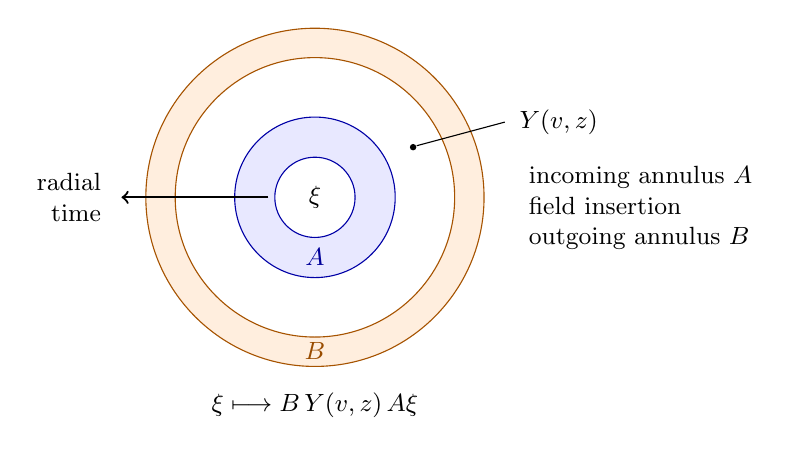
\begin{tikzpicture}[scale=0.91, font=\small]
  \fill[blue!9,even odd rule] (0,0) circle (1.12) (0,0) circle (0.56);
  \fill[orange!13,even odd rule] (0,0) circle (2.36) (0,0) circle (1.95);
  \draw[blue!65!black] (0,0) circle (0.56);
  \draw[blue!65!black] (0,0) circle (1.12);
  \draw[orange!65!black] (0,0) circle (1.95);
  \draw[orange!65!black] (0,0) circle (2.36);
  \node at (0,0) {$\xi$};
  \node[blue!60!black] at (0,-0.83) {$A$};
  \node[orange!60!black] at (0,-2.15) {$B$};
  \fill (1.37,0.70) circle (0.045);
  \draw (1.42,0.72) -- (2.65,1.05);
  \node[anchor=west] at (2.72,1.05) {$Y(v,z)$};
  \draw[->,thick] (-0.65,0) -- (-2.70,0);
  \node[anchor=east,align=right] at (-2.85,0)
       {radial\\time};
  \node[anchor=west,align=left] at (2.85,-0.15)
       {incoming annulus $A$\\field insertion\\outgoing annulus $B$};
  \node at (0,-2.9) {$\displaystyle \xi\longmapsto B\,Y(v,z)\,A\xi$};
\end{tikzpicture}

\caption{Radial ordering of a regularized insertion. The inner
annulus prepares the input, the field lies in the intervening
region, and the outer annulus regularizes the output. This round
schematic illustrates the order $BYA$; actual geometric annuli
need not be concentric, and boundedness requires the analytic
insertion theorem rather than the picture alone.}
\label{fig:unitarity-annuli}
\end{figure}

\begin{example}[Energy damping in one oscillator]
Let $a^\dagger|n\rangle=\sqrt{n+1}|n+1\rangle$ on an oscillator
Hilbert space and $N|n\rangle=n|n\rangle$.
The operator $a^\dagger$ is unbounded, but
$a^\dagger r^N$ is bounded because
\[
 \norm{a^\dagger r^N}^2
 =\sup_{n\ge0}(n+1)r^{2n}<\infty.
\]
Exponential damping beats polynomial growth. The annulus argument
is a geometric and many-field version of this mechanism.
The inverse $r^{-N}$ remains unbounded; density arguments must
therefore be stated with their domains.
\end{example}

\begin{lemma}[A dense domain for undoing an incoming annulus]
\label{lem:unitarity-annulus-domain}
Suppose $A,C$ are bounded injective annulus operators with dense
range, and $AC=\lambda r^{L_0}$ with $\lambda\ne0$, $0<r<1$.
On an ordinary module,
$M^{\rm fin}\subset\operatorname{Ran}A$ and
$A^{-1}M^{\rm fin}=CM^{\rm fin}$ is dense, where
$M^{\rm fin}$ is the algebraic finite-energy space and the
inverse is taken only on $\operatorname{Ran}A$.
\end{lemma}
\begin{proof}
For a finite-energy vector $v$, $r^{-L_0}v$ is again a finite
vector, so $v=AC\lambda^{-1}r^{-L_0}v$ lies in $\operatorname{Ran}A$.
Injectivity of $A$ then gives
$A^{-1}M^{\rm fin}=CM^{\rm fin}$. The right side is dense because
$M^{\rm fin}$ is dense and $C$ is bounded with dense range.
\end{proof}

The chosen geometric annuli satisfy these hypotheses. The
inner Jordan domain of an incoming annulus contains the origin.
Place a sufficiently small round disc $r\mathbb D$ inside that
domain and choose the intervening annulus $C$, with matching
boundary parametrizations. Sewing $A$ and $C$ gives the round
annulus, so its central lift yields $AC=\lambda r^{L_0}$.
The geometric annulus theorem supplies injectivity and dense
range for both factors. The outgoing adjoint admits the same
construction. Thus the lemma verifies actual range and density
conditions needed below.

When both test vectors become finite-energy after the incoming
and outgoing annulus actions, their formal field matrix element is
a finite Laurent polynomial. For an input energy $p$, output
energy $q$, and field weight $k$, only the mode
$n=p+k-q-1$ contributes. This elementary grading observation allows
analytic continuation of matrix coefficients through the insertion
interior. Here is the geometric detail behind this continuation.
Write
\[
 D_A=\{\xi:A_M\xi\in M^{\rm fin}\},\qquad
 D_{B^*}=\{\eta:B_M^*\eta\in M^{\rm fin}\}.
\]
Both are dense by the preceding lemma and its outgoing analogue.
For one geometric representative of the pair, let
$O_{\rm in},O_{\rm out}$ be the incoming and outgoing comparison
regions and put
\[
\Omega_{\rm ins}=\operatorname{int}
   \bigl(\overline{O_{\rm in}}\cup\overline{O_{\rm out}}\bigr).
\]
The geometric point-insertion theorem supplies a bounded operator
$G_v(z)$ whose matrix coefficients are holomorphic on this
domain, which lies in $\C^\times$. The finite-Laurent
coefficient is holomorphic there as well.
Every component of $\Omega_{\rm ins}$ meets
$O_{\rm in}\cup O_{\rm out}$: the part omitted from this union
lies in two nowhere-dense boundaries and cannot contain a component,
which is open. The identity theorem therefore extends each tested
finite-Laurent coefficient throughout that component. Repeat for
the geometric representatives; the prescribed insertion interior
is the union of their allowed interiors. Boundedness and the dense test domains make
these continuations unique on overlaps. The argument compares
bounded extensions of sesquilinear forms; it does not assume that
an unsmeared field is defined on every Hilbert-space vector.

\section{Why paired lifts matter}
\index{deck transformation}\index{Haag duality}

Annulus and diffeomorphism actions involve central extensions.
A full rotation acts on a simple ordinary module of lowest weight $h$ by
$Z=e^{2\pi iL_0}=e^{2\pi ih}$, while it acts trivially on the
integer-graded vacuum VOA. Consequently two geometric lifts can
agree in the vacuum and still differ by a nontrivial phase in a
charged sector. Normalizing a vacuum scalar cannot erase that
ambiguity.

The comparison used here chooses lifts for an incoming--outgoing
pair after localizing both with one common diffeomorphism. Undoing
that common lift gives actions $A_M,B_M$ in each sector.
More explicitly, choose a common localizer $\delta$ so that
$\mathsf U_U(\delta)A_U$ and $B_U\mathsf U_U(\delta)^*$
belong to the interval algebra. With one lift $\widetilde\delta$,
the actions are
\begin{align*}
 A_M&=\mathsf U_M(\widetilde\delta)^*
       \pi_M\!\left(\mathsf U_U(\delta)A_U\right),\\
 B_M&=\pi_M\!\left(B_U\mathsf U_U(\delta)^*\right)
       \mathsf U_M(\widetilde\delta).
\end{align*}
Here $\mathsf U$ denotes diffeomorphism action, not the VOA $U$, and
$\pi_M$ is the net representation on the Hilbert completion of $M$.
The geometric comparison matches the incoming annulus
parametrization and its central normalization as part of this
construction. Changing
the common lift by $Z^m$ changes the pair to
\[
 A_M\longmapsto Z^{-m}A_M,\qquad
 B_M\longmapsto B_MZ^m.
\]
Every $U$-mode shifts energy by an integer, so it commutes with
$Z$. The regularized insertion is unchanged. This cancellation
uses the pair; it does not require a global choice of lift for
each individual annulus.

The resulting specific comparison identity is
\begin{equation}
 \pi_M\bigl(X_v(B,z,A)\bigr)
   =\overline{B_MY_M(v,z)A_M}.
 \label{eq:unitarity-pair-comparison}
\end{equation}
The geometric transport theorem proves it first in the incoming
interior, the adjoint identity proves the outgoing version, and
the finite-Laurent continuation proves it on the full allowed
interior. Empty-interior pairs are covered by the no-insertion
identity $\pi_M(BA)=B_MA_M$. On the vacuum space, locality and
Haag duality then identify the concrete bounded-insertion and
smeared-field nets. Write $\mathcal A_{\rm bl}$ for the
bounded-insertion vacuum net. Haag duality says that the algebra of an
interval is exactly the commutant of the complementary interval's
algebra, in the vacuum representation. On the common vacuum Hilbert space the
argument is the chain
\[
 \mathcal A_{\rm bl}(I)\subset\mathcal N_U(I)
 \subset\mathcal A_{\rm bl}(I')'
 =\mathcal A_{\rm bl}(I).
\]
The first inclusion is the comparison just proved; the second
uses locality and the first inclusion at $I'$; the equality uses
Haag duality of the conformal vacuum net $\mathcal A_{\rm bl}$.
Thus the conclusion identifies the actual algebras.

\section{The final positivity implication and its scope}

The fusion-positivity theorem applies to a simple regular unitary
VOA with bounded localized vertex operators, provided every
ordinary module is unitarizable and has the corresponding net
representation. These hypotheses are now established for $U$:
strong unitarity supplies the positive modules, and their
representations satisfy
\eqref{eq:unitarity-pair-comparison}. It gives positivity of the
canonical fusion forms. Thus the construction concludes that $U$
is completely unitary, under the preceding finite construction
inputs and structural and analytic theorems.

Now the actual extension algebra can be treated as a positive
Q-system. Its category of all modules is a unitary fusion category
with the already determined Haagerup--Izumi ring and untwisted
pointed subcategory. The unitary classification gives the two
possibilities $\mathcal H_2$ and $\mathcal H_3$. Their Morita
equivalence identifies their centers, so
\[
 \Rep(U)\simeq Z(\mathcal H_3)
\]
as unitary ribbon categories. This conclusion uses the unitary
classification and center correspondence, rather than asserting
that a natural linear reconstruction functor has already been
proved to preserve every tensor operation.

For the original embedded $E_8/U$ extension, the boundary category
may be $\mathcal H_2$ or $\mathcal H_3$. To obtain a specified
$\mathcal H_3$ extension, transport its canonical Lagrangian
Q-system along the center equivalence. The positive extension
correspondence then gives a holomorphic strongly rational unitary
VOA of central charge eight, which the central-charge-eight holomorphic VOA classification
identifies with $V_{E_8}$. Isomorphism of the ambient holomorphic
VOAs does not identify their embeddings of $U$.

The net-side diagonal full theory has a route using complete
rationality and sector reconstruction before the final fusion-form
comparison. The specified VOA extension uses the stronger
complete-unitarity conclusion. Distinguishing these routes explains
which claims survive if a particular analytic comparison is under
review, and prevents one construction from being used circularly
to prove its own hypotheses.

\section{Exercises}

\begin{exercise}\label{ex:unitarity-damping}
For $0<r<1$, bound $\sup_{n\ge0}(n+1)r^{2n}$ explicitly using
the corresponding function on $x\ge0$. Show why the bound diverges
as $r\to1$.

\par\smallskip\noindent{\footnotesize\normalfont
\hyperref[sol:ex:unitarity-damping]{Solution on page~\pageref*{sol:ex:unitarity-damping}.}}\par
\end{exercise}

\begin{exercise}\label{ex:unitarity-projector}
Prove Lemma~\ref{lem:unitarity-core} for the complementary
projection $1-P$ and explain exactly where it is used to obtain
a statement about $T^*$.

\par\smallskip\noindent{\footnotesize\normalfont
\hyperref[sol:ex:unitarity-projector]{Solution on page~\pageref*{sol:ex:unitarity-projector}.}}\par
\end{exercise}

\begin{exercise}\label{ex:unitarity-counting}
A fully faithful linear functor sends twelve simple objects into a
semisimple category with twelve simples. Prove essential
surjectivity on finite direct sums. Explain why the same argument
does not construct a tensorator.

\par\smallskip\noindent{\footnotesize\normalfont
\hyperref[sol:ex:unitarity-counting]{Solution on page~\pageref*{sol:ex:unitarity-counting}.}}\par
\end{exercise}

\begin{exercise}\label{ex:unitarity-deck}
On a module with $h=1/3$, compute the phase of a full rotation.
Show that it is invisible on the vacuum and cancels in
$BZ^mY(v,z)Z^{-m}A$ for $v\in U$. What grading property is needed?

\par\smallskip\noindent{\footnotesize\normalfont
\hyperref[sol:ex:unitarity-deck]{Solution on page~\pageref*{sol:ex:unitarity-deck}.}}\par
\end{exercise}

\begin{exercise}\label{ex:unitarity-end}
If an extension restricts as
$\one\oplus X\oplus Y\oplus Y^*$, compute its endomorphism
algebra when $Y\not\cong Y^*$ and when $Y\cong Y^*$, assuming
the named simple objects are otherwise distinct. Relate the
dimensions to the rank-four/rank-six alternatives.

\par\smallskip\noindent{\footnotesize\normalfont
\hyperref[sol:ex:unitarity-end]{Solution on page~\pageref*{sol:ex:unitarity-end}.}}\par
\end{exercise}
